\documentclass[12pt]{article}
\usepackage{epsfig}
\usepackage{graphicx}
\usepackage{color}
\usepackage[frenchb]{babel}
\usepackage{subfigure}
\usepackage{amsmath}
\usepackage{amssymb}
\usepackage{enumerate}

% Pour pouvoir utiliser les accents directement dans LaTeX, sans utiliser les commandes \'
%\usepackage[latin1]{inputenc} % entree 8 bits iso-latin1
\usepackage[utf8]{inputenc} % entree 8 bits utf8, fonctionne avec MikTeX sur Windows.
\usepackage[T1]{fontenc}      % encodage 8 bits des fontes utilisees

% Pour agrandir les marges
\addtolength{\oddsidemargin}{-.875in}
\addtolength{\evensidemargin}{-.875in}
\addtolength{\textwidth}{1.75in}
\addtolength{\topmargin}{-.875in}
\addtolength{\textheight}{1.75in}

\begin{document}
\selectlanguage{french}
\title{Introduction à la robotique mobile : travail pratique 3  \\  Date de remise : 8 décembre 2017, 23h55.}
%\subtitle{Travail Pratique No 1}
\author{Instructeur : Philippe Giguère}

\maketitle

\section{Instructions générales}
Ce travail pratique se fait en équipe de 1 à 2. Dans l'évaluation du rapport, 10 points seront attribués à la qualité de la présentation. Les critères d'évaluations seront :
\begin{itemize}
\item la qualité du français;
\item la propreté de la présentation;
\item le degré d'élaboration et la présentation structurée des réponses : évitez donc de simplement donner la réponse sans un minimum de discussion;
\end{itemize}
N'oubliez pas d'inclure TOUS les scripts/fonctions dans le fichier .zip. Vous pouvez faire le TP en matlab ou en python. Malheureusement, je ne peux fournir de fichiers scripts pour Python.
\vspace{1in}

Pour les étudiants en GLO-7021, le rapport doit être rédigé sur Latex.

% ========================= D e s c r i p t i o n    P r o b l è m e  =========================
\newpage
\section {Description d'un problème d'estimation d'état}
\label{DescriptionProbleme}

\begin{figure}[ht]
 \begin{center}
  \begin{tabular}{c}
    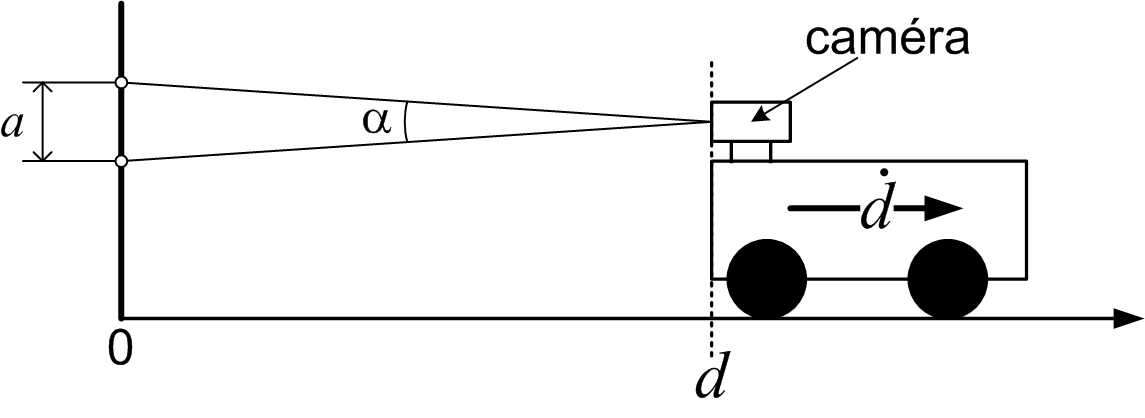
\includegraphics[width=0.60\textwidth]{ChariotCamera.png}
  \end{tabular}
 \end{center}
 \vspace{-0.3in}
 \caption{Chariot motorisé équipé d'une caméra mesurant un angle $\alpha$.}
 \label{Chariot}
\end{figure}

Vous avez un chariot motorisé, tel qu'illustré à la Fig. \ref{Chariot}. Le chariot possède une caméra qui mesure $\alpha$, entre des marqueurs placés sur le mur. La fonction du capteur non-linéaire sera :
\begin{equation}
\alpha = h_z(d) = \frac{0.07}{d}
\label{Mesure}
\end{equation}
où $d$ est la distance en mètre entre le robot et le chariot. Le bruit sur cette mesure a un écart-type de $\sigma_{z}=0.003$. Le capteur n'est pas biaisé, et il n'y a jamais d'obstacles entre le robot et les marqueurs sur le mur.
La commande de voltage du moteur $u$ est :
\begin{equation}
u(t) = 8\sin(0.2\pi t) \mbox{ (en Volt)}
\label{Commande}
\end{equation}
La relation entre le voltage $u$ du moteur (en V) et la vitesse $\dot{d}$ du chariot (en $m/s$) est non-linéaire, et correspond (pour les besoins de la cause\footnote{Cette courbe n'est pas du tout réelle, mais seulement pour avoir une fonction non-linéaire facile à exprimer.}) à la fonction suivante :
\begin{equation}
\dot{d} = 2(\frac{1}{1+e^{-u/2}}-0.5)
\label{VtoSpeed}
\end{equation}
Cette relation est illustrée à la Fig. \ref{CurveVolt}. L'écart-type du bruit sur la commande de voltage $u$ est $\sigma_u=0.15$ $V$.

\begin{figure}[ht]
 \begin{center}
  \begin{tabular}{c}
    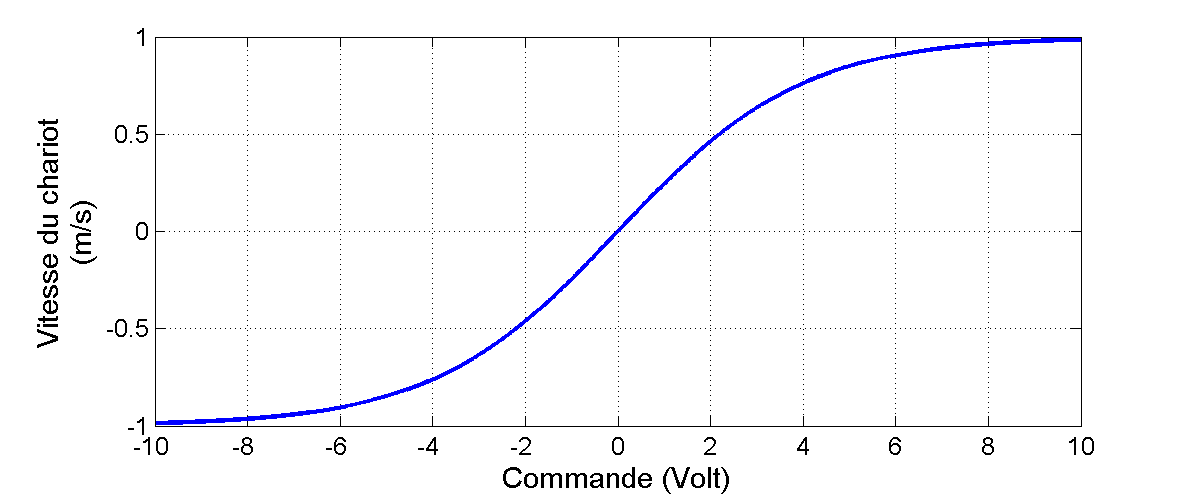
\includegraphics[width=0.64\textwidth]{CurveVolt.png}
  \end{tabular}
 \end{center}
 \vspace{-0.3in}
 \caption{Courbe de l'équation \ref{VtoSpeed} reliant le voltage $u$ du moteur à la vitesse linéaire $\dot{d}$ du chariot.}
 \label{CurveVolt}
\end{figure}
L'état du robot dans ce monde à une dimension est défini par :
\begin{equation}
X = \begin{bmatrix}
d  \\
\dot{d}   \\
\end{bmatrix}
\end{equation}
où $\dot{d}$ est la vitesse du robot. Au départ, le robot est placé à $d_{init}=3$ $m$, et le chariot est au repos, i.e $\dot{d}=0$. Le code matlab fourni \texttt{Chariot.m} utilise $\Delta t=0.1~s$, ce qui signifie que les déplacements sont effectués et les mesures sont prises à chaque $\Delta t$. Ce même code calcule la commande (Eq.~\ref{Commande}), la position réelle du chariot et simule les mesures (Eq.~\ref{Mesure}) pour ces positions réelles.

% =========================   F i l t r e   à   p a r t i c u l e s   =========================
\section {Solution par filtre à particules (10 pts)}
\label{Particules}
Afin de vous familiariser avec la notion de filtrage, faites un filtre à particules pour le problème décrit à la section \ref{DescriptionProbleme}, à partir d'une copie du fichier \texttt{Chariot.m} et du code fournis sur le site web du cours pour les filtres à particules. Pour ce filtre, utilisez les paramètres suivants :
\begin{itemize}
\item $C$ = 40 particules; Dans le code, \texttt{nParticules} = $C$.
\item Ratio effectif $C/N_{eff}$ = $R_{eff} = 0.5$
\end{itemize}

Pour l'estimé de la position $d$, prenez la moyenne pondérée des particules : \texttt{Xmoyen = sum(X(1,:).*w);} Testez votre filtre à particules pour 400 itérations (donc de $t=0$ $s$ à $t=40$ $s$) uniquement pour le cas où vous connaissez exactement la position initiale du robot au départ. Vous initialisez donc toutes les particules avec $X=[d_{init} \mbox{ }0]^T$.

Note : le filtre à particules n'est pas nécessairement la meilleure solution pour ce problème, car la distribution des croyances sur l'état est unimodale. Cependant, l'implémentation est plus facile à faire et à débugger qu'un filtre EKF, et cela vous permettra en quelque sorte de vérifier que toutes les équations du systèmes sont les bonnes. D'ailleurs, ces équations vous sont essentiellement données dans \texttt{Chariot.m}, car il simule déjà le système ;).


% =========================   E K F  =========================
\newpage
\section{Filtre Kalman étendu (EKF) (40 pts pour GLO-4001, 35 pts pour GLO-7021)}
\label{EKF}
\subsection{Matrices Jacobiennes (10 pts)}
La matrice $\Phi$ du système est
\begin{equation}
\Phi = \begin{bmatrix}
1 &  \Delta t  \\
0  &  0     \\
\end{bmatrix}
\end{equation}

Quelles sont les matrices jacobiennes de commande $\Gamma$ et de mesure $\Lambda$ pour ce système? Important! La matrice $\Gamma$ est utilisée pour propager le bruit de moteur en Volt vers des $m/s$.

\subsubsection{Détermination de $\Gamma$}
Soit nous définissons $\Gamma$ comme la matrice de dérivé des fonctions de mesure selon la commande:
\begin{equation}
\Gamma =
\begin{bmatrix}
    0   \\
    \\
    \dfrac{\exp(-u/2)}{(1+\exp(-u/2))^2} \\
\end{bmatrix}
\end{equation}

\subsubsection{Détermination de $\Lambda$}
\begin{equation}
\Lambda =
\begin{bmatrix}
    \frac{-0.07}{d^2}   \\
    0
\end{bmatrix}
\end{equation}


\subsection{Implémentation du filtre EKF (30 pts pour GLO-4001, 25 pts pour GLO-7021)}
Implémentez le filtre de Kalman étendu (EKF) à partir d'une copie du fichier incomplet matlab \texttt{Chariot.m} pour estimer la position $d$ du robot\footnote{Attention! pour ceux qui feront le code en python, méfiez-vous de l'opérateur \texttt{*}, car il peut donner l'impression que c'est une multiplication de matrices, alors que dans les faits c'est une multiplication entrée-par-entrée pour des \texttt{Array} et matricielle pour des \texttt{numpy.matrix}. Bref, un beau piège subtil...}. Testez votre filtre de Kalman pour 400 itérations (donc de $t=0$~$s$ à $t=40$~$s$), avec les scénarios suivants :
\begin{enumerate}[a)]
\item Vous connaissez exactement la position initiale du robot au départ. Vous initialisez donc la matrice d'état à $X=[d_{init} \mbox{ }0]^T$, et la matrice de covariance à
$$
P=
\begin{bmatrix}
0 &0\\
0 & 0
\end{bmatrix}
$$

\item Vous avez une bonne idée de la position initiale du robot au départ, mais vous n'êtes pas confiant à $100~\%$. Vous initialisez donc la matrice d'état à $X=[d_{init} \mbox{ }0]^T$, et la matrice de covariance à
$$
P=
\begin{bmatrix}
25 &0\\
0 & 1
\end{bmatrix}
$$

\item Vous croyez connaitre exactement la position initiale du robot au départ, mais cette valeur est, dans les faits, erronée. Vous initialisez donc la matrice d'état à $X=[(d_{init}+1) \mbox{  } 0]^T$, et la matrice de covariance à
$$
P=
\begin{bmatrix}
0 &0\\
0 & 0
\end{bmatrix}
$$

\item Vous n'êtes pas sûr que $d=d_{init}+1$ est la bonne position de départ du chariot. Vous initialisez donc la matrice d'état à $X=[(d_{init}+1)  \mbox{  }  0]^T$, et la matrice de covariance reflète cette incertitude car vous l'initialisez à:
$$
P=
\begin{bmatrix}
100 &0\\
0 & 1
\end{bmatrix}
$$

\end{enumerate}

Pour tous les cas a)-d), décrivez le comportement de l'estimé de la position $X(1)$ du filtre EKF en quelques lignes, en portant une attention particulière à :
\begin{itemize}
\item l'erreur au début ($t<0.5~s$) du filtrage;
\item l'erreur moyenne;
\item la vitesse de convergence (ou non) de l'estimé vers la valeur réelle, surtout au début.
\end{itemize}
Faites quelques essais pour trouver des simulations concluantes\footnote{par exemple, si la première mesure est très erronée et que votre matrice de covariance $P$ indique une grande incertitude, vous allez voir une grande correction pour cette simulation.}. Incluez pour chacun des cas a)-d) un graphique pour l'une de ces simulations concluantes montrant, en fonction du temps :
\begin{itemize}
\item la position réelle du chariot avec le paramètre \texttt{'k-'} dans \texttt{plot};
\item la position estimée $X(1)$ du chariot avec le paramètre \texttt{'go'} dans \texttt{plot};
\item la position correspondant à la mesure inversée $d=h_z^{-1}(z)$ du chariot  avec le paramètre \texttt{'r*'} dans \texttt{plot}.
\end{itemize}
Notez que le code matlab inclus dans le TP fait déjà ces graphiques pour vous.

%Pour le cas a), rapportez aussi :
%\begin{itemize}
%\item l'écart-type sur l'erreur entre la position estimée $X(1)$  dans l'EKF et la position véritable;
%\item l'écart-type sur l'erreur entre la position mesurée $d_z=h_z^{-1}(z)$  et la position véritable;
%\end{itemize}


% =========================   F i l t r e   à   p a r t i c u l e s   =========================
\newpage
\section {Localisation globale par filtre à particules (35 pts)}
\label{LocalisationGlobale}
Vous avez un robot initialement perdu, dans un environnement dont la carte est connue. Pour pouvoir le localiser, vous devrez donc utiliser un filtre à particules, puisque la distribution de croyance sur l'état du robot sera mulitmodale. Un aspect important de la question sera de trouver des bons paramètres, pour permettre au système de se localiser de manière robuste. Notez ici que nous ne chercherons pas à faire une solution qui puisse tourner en temps-réel; ne vous préoccupez donc pas d'optimiser le code pour sa vitesse d'exécution.

Pour tous les cas, nous allons utiliser le même monde qu'au TP1, c'est à dire un monde décrit par un polygone et contenu dans le fichier \texttt{Carte.mat}. Le robot ponctuel (rayon=0) est équipé de 4 LiDAR, pointant dans les directions 0, $\pi/2$,  $\pi$ et $1.5\pi$, tel qu'illustré à la Fig.~\ref{CartePlusRobotLiDAR}. Le robot est soumis aux bruits gaussiens suivants (avec les noms de variable entre parenthèses) :
\begin{itemize}
\item LiDAR (\texttt{Lidar}) : $\sigma_{L}=0.01$ $m$;
\item Vitesse linéaire (\texttt{V}): $\sigma_{V}=0.01$ $m/s$;
\item Vitesse angulaire (\texttt{omega}) : $\sigma_{\omega}=0.05$ $rad/s$;
\item Compas magnétique  (\texttt{Compas}) : $\sigma_{C}=0.01$ $rad$.
\end{itemize}

\begin{figure}[ht]
 \begin{center}
  \begin{tabular}{c}
    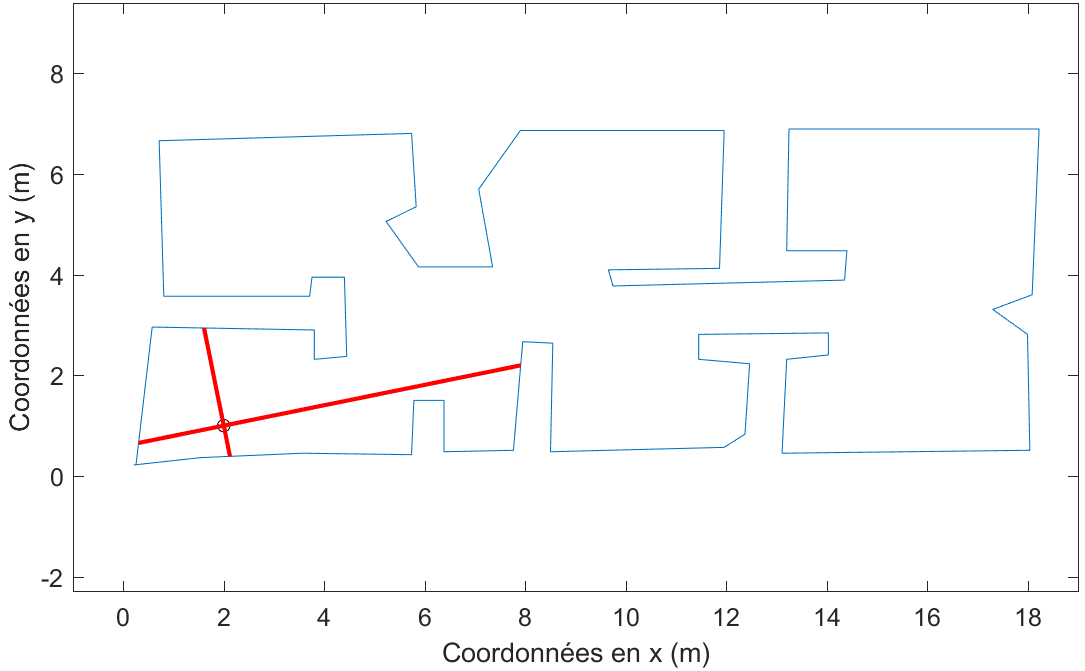
\includegraphics[width=0.65\textwidth]{CartePlusRobotLiDAR.png}
  \end{tabular}
 \end{center}
 \vspace{-0.3in}
 \caption{Robot ponctuel dans un environnement décrit par un polygone identique au TP1. Les 4 lignes rouges indiquent les faisceaux laser.}
 \label{CartePlusRobotLiDAR}
\end{figure}

Pour prédire les mesures LiDAR, vous allez utiliser des fonctions géométriques. Le faisceau LiDAR sera simplement un segment de droite partant du centre du robot et allant à une distance maximale (disons 20~$m$), selon l'angle du LiDAR (et bien sûr l'angle du robot, puisque le LiDAR est fixé sur ce dernier). Trouvez tous les points de cette droite qui interceptent le polygone de la carte (fonction \texttt{polyxpoly} dans matlab, ou la fonction appropriée dans le package  \texttt{Shapely} dans Python).  La distance mesurée par le LiDAR sera celle correspondante au point le plus proche du centre du robot.

Pour l'initialisation des particules, vous pouvez les distribuer de manière uniforme dans un rectangle couvrant la carte au complet. Ne vous préoccupez pas des particules en dehors du polygone (essentiellement en dehors de l'environnement). Ils finiront par avoir des poids quasi-nuls et seront donc éliminé lors de la phase du resampling. (Si vous insistez, la fonction \texttt{inpolygon} permet de trouver les points à l'intérieur d'un polygone. D'ailleurs, il serait en théorie possible de se localiser uniquement à partir de cette contrainte. Mais je diverge...)

\subsection{Cas 1 : l'angle est connu (GLO-4001 : 30 pts, GLO-7021 : 20 pts)}
\label{Q1Global}
Afin d'y aller en douceur, nous allons commencer par un problème d'estimation à deux dimensions, où l'état est simplement $X=[x\mbox{ } y]^T$. Pour l'angle du robot, vous allez simplement prendre l'angle \texttt{Compas} mesuré par le compas magnétique (en rad, de $-\pi$ à $\pi$), et ajouter un bruit $\sigma_{angle}$ aléatoire sur l'angle. Ce bruit permettra de ``brasser'' les particules un peu, pour permettre une convergence plus rapide, en plus de tenir compte de l'incertitude du compas.  Faites un filtre à particules qui exploite les informations suivantes :
\begin{itemize}
\item les 4 mesures LiDAR (\texttt{Lidar}), en $m$;
\item la vitesse linéaire (\texttt{V}), en $m/s$;
\item l'angle du compas magnétique  (\texttt{Compas}), en $rad$.
\end{itemize}

\vspace{0.1in}
Dans votre rapport, discutez des éléments suivants :
\begin{itemize}
\item une justification de votre choix $\sigma_{angle}$;
\item les divers paramètres utilisés dans le filtre (pour GLO-7021, la question \ref{ImpactLidarBruit} vous demande d'élaborer sur certains de ces paramètres, alors ne pas dupliquer);
\item description qualitative de la distribution des particules au fil du temps.
\end{itemize}

Incluez deux tracés de trajectoires estimées par votre filtre, l'une pour une exécution réussie du filtre et l'autre pour une exécution qui n'a pas convergée. La  trajectoire est basée sur le calcul, à chaque itération, de la moyenne des particules (pondérée par leur poids respectif). Dans le cas où le filtre a échoué, donnez une explication qualitative.

Pour les étudiants de GLO-7020, votre note dépendra de la qualité des explications et justifications. Par exemple, il serait intéressant de voir des graphiques d'erreur en fonction du temps vs. choix de  $\sigma_{angle}$.

\begin{center}
\textbf{Pour les étudiants en GLO-4001, le TP se termine ici!}
\end{center}

\newpage
\subsection{Impact du bruit utilisé dans la vraisemblance LiDAR (GLO-7021 seulement, 10 pts)}
\label{ImpactLidarBruit}
Lors de la mise-à-jour, vous devez choisir l'écart-type $\sigma_{LiDAR}$ pour évaluer la vraisemblance des mesures du LiDAR dans la fonction $p(z|x)$. Quel est l'impact de cette valeur, en terme \emph{a)} du nombre de particules nécessaire pour converger et \emph{b)} de la vitesse de convergence du filtre. Pour\emph{a)}, faites 10 essais par nombre de particules, et rapportez le pourcentage de succès. Vous devrez trouver, par essai et erreur, des valeurs ``intéressantes'' de nombres de particules pour ces tests, i.e. pour lesquels le taux de succès change. Pour aller plus vite, ne laissez pas tourner le filtre sur toutes les itérations : dès que vous voyez que les particules ont condensé en une région, vous pouvez établir si le filtre a divergé ou non par rapport à la vérité-terrain.

Prenez des mesures sur la vitesse d'appauvrissement, afin de voir l'impact de $\sigma_{LiDAR}$ sur cette vitesse.

 Selon vos résultats, en quoi serait-il intéressant d'augmenter ou de diminuer graduellement $\sigma_{LiDAR}$ au fil du temps? Si vous comprenez bien cette question, cela vous sera utile pour la question \ref{Q2Global} pour accélérer le filtrage.

\subsection{Cas 2 : l'angle est inconnu (GLO-7021 Seulement, 25 pts)}
\label{Q2Global}
Pour ce cas-ci, la dimensionalité du problème va augmenter, car il vous faudra maintenant estimer l'état en y incluant l'angle $\theta$ du robot : $X=[x \mbox{ } y \mbox{ } \theta]^T$. Tel que vu en classe, le nombre de particules est exponentiel en dimension de l'état... Alors vous devrez probablement être patient lors de l'exécution de votre filtre! Le fichier de donnée pour ce cas d'estimation, \texttt{Q2Trajectoire.mat}, contient les commandes de vitesses linéaires et les commandes angulaires, les mesures LiDAR et la vérité-terrain. Notez ici que vous n'avez plus de données du compas. Vous pouvez partir de votre implémentation du filtre à particule de la section~\ref{Q1Global}.

Refaites les mêmes expérience qu'à la section \ref{ImpactLidarBruit} et commentez sur ces résultats.

À partir de votre expérience de l'impact de $\sigma_{LiDAR}$ et du nombre de particules sur les chances de convergences, adaptez ces valeurs dynamiquement afin d'accélérer l'exécution du filtre à particules. Expliquez votre stratégies, notamment à l'aide de graphiques montrant le nombre de particules, la valeur de $\sigma_{LiDAR}$ et les erreur en distance/orientation en fonction du temps. Appuyez ausis votre réponse avec des histogrammes d'erreur correspondant au régime pour lequel le filtre a convergé.

Comment pouvez-vous justifier votre approche, d'un point de vue théorique?

\end{document}
